%% \subsection{Push and Pull}
%% \label{subsec:ADSL_Elements_SAL}

\vatsan{Should we "add" a discussion on Program Counter (PCs) in addition to "mutex" discussion below. Then we discuss the reason for doing as controlling state exploration of model checker along time domain and space/value domain through these "primitives". Thereby we have a chance to have "scalable" model checking}

\begin{figure}
\begin{tabular}{cc}
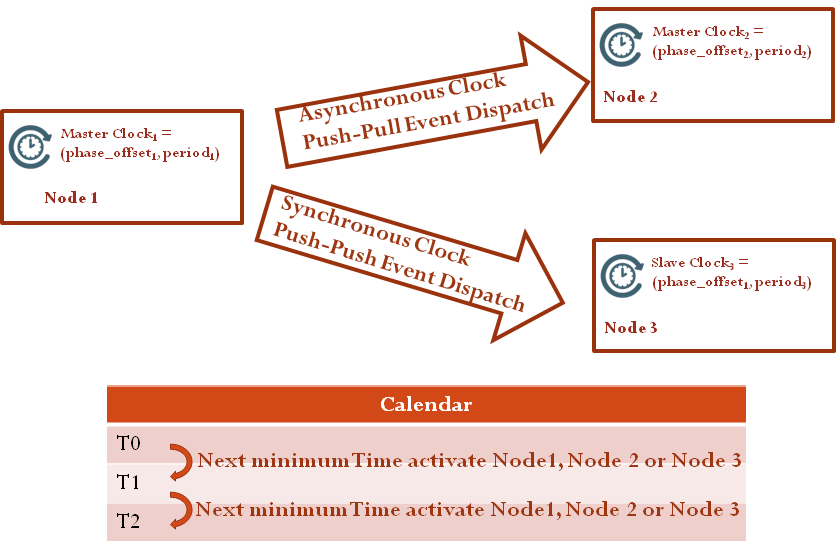
\includegraphics[width=0.7\textwidth]{figures/three_node.png}\\ 
(a) 3 Node Scenario\\ \\ \\
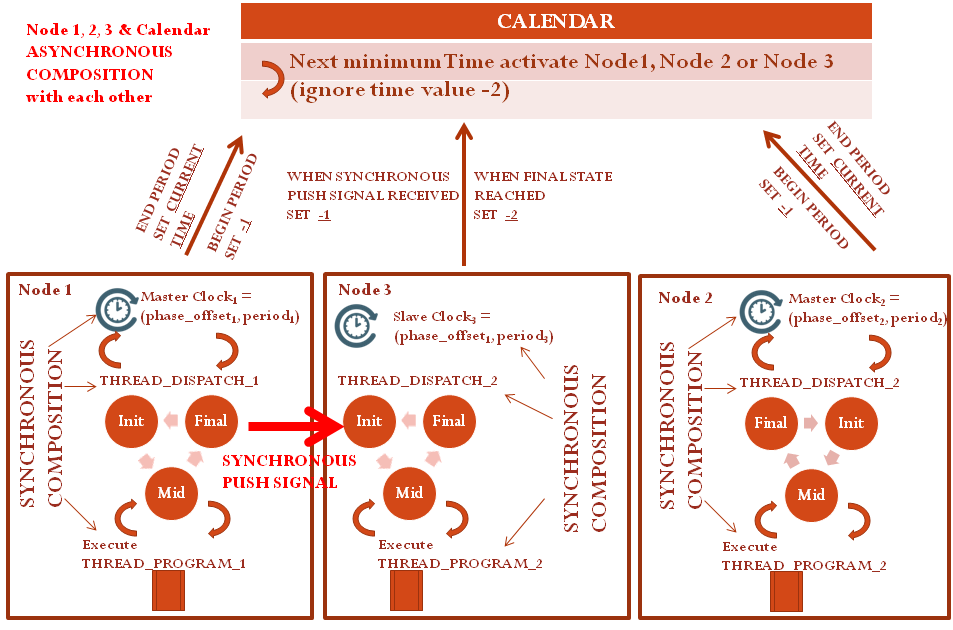
\includegraphics[width=0.9\textwidth]{figures/three_node_sal.png}\\ 
 (b) SAL Model \\
\end{tabular}
\caption{Synchronous \& Asynchronous Clock Models Implemented in ADSL Target}
\label{fig:clock_models_sal}
\end{figure}

%% Here we model the \emph{synchronous} and \emph{asynchronous} mode of
%% interactions between different nodes and their associated clocks described in
%% Section~\ref{subsec:ADSL_Elements}. The SAL code then is the anticipated ADSL
%% target we hope to synthesize in our ADSL workbench when the corresponding
%% synchronous and asynchronous clocks are specified in the ADSL.

Let us provide a concrete example. As shown in
Figure~\ref{fig:clock_models_sal}(a), we consider a three node scenario where
$Node1$ is a producer/transmitter and $Node2$ and $Node3$ are
consumers/receivers. $Node1 \Longrightarrow Node 2$ is an \emph{asynchronous}
mode of interaction between two master clocks $Clock_1$ and $Clock_2$. Thus the
event dispatch model is \emph{push-pull}. But $Node1 \Longrightarrow Node 3$ is
an \emph{synchronous} mode of interaction between master clock $Clock_1$ and
slave $Clock_3$ with event dispatch model being \emph{push-push}. Also for the
moment we ignore modeling slave $Clock_3$ and the model can trivially be
extended to include the same. Notice that we model both synchronous and
asynchronous clocks dispatch event semantics in a single SAL model. This then
provides an opportunity in the framework to model in the future even transitions
from Sync to Async and vice-versa which will be immensely useful in also
modeling Start-up and Synchronization protocol (e.g. TTE). We
have also kept the code “minimal” with reference to variables that will be used
and explored in the model checker so as to reduce the risk of “scalability”
issues of proofs when using this SAL code as building blocks for larger models.

A calendar automata keeps track of the "next" minimum time with which to
activate $Node1$, $Node2$ and $Node3$. The
minimum time tracked by the calendar is shown in code below lines $8-19,
11-12$. Time $t = -2$ “special case” (\textcolor{red}{line $9$}) for
\emph{out-of-band signaling to calendar} to handle synchronous push at
$Node3$. Calendar “ignores” value -2 and is then used by nodes (like $Node3$) to
\emph{expire} time events after handling/processing of synchronous push
events. This is also shown in the CA at the top of
Figure~\ref{fig:clock_models_sal}(b). Further $Node1$, $Node2$, $Node3$ and CA
are asynchronously composed with each other (lines $14-21$). Boolean signal
“thread1\_push\_thread3\_signal” pushed from $Node1$ as
“producer\_signal\_event” in $Node3$ (\textcolor{red}{line $21$}).  This signal
in essence captures the synchronous \emph{push-push} event dispatch discussed in
Section~\ref{subsec:ADSL_Elements} and is also illustrated in
\ref{fig:clock_models_sal}(b) between $Node1$ and $Node3$.

\begin{figure}[ht]
\centering
\begin{sal}
N : NATURAL = 3; TIME : TYPE = REAL; THREAD_NUM : TYPE = [1 .. N]; TIMEOUT_ARR :
TYPE = ARRAY THREAD_NUM OF TIME;

THREAD1_PERIOD : TIME = 10; THREAD2_PERIOD : TIME = 20;

THREAD_STATE : TYPE = {THREAD_INIT, THREAD_MID, THREAD_FINAL};

is_min(x : TIMEOUT_ARR, t : TIME) : bool = (FORALL (i: THREAD_NUM) : t <= x[i])
  AND (EXISTS (i: THREAD_NUM) : t = x[i]) AND (@t /= -2@);

Calendar : MODULE = BEGIN INPUT time_arr : TIMEOUT_ARR OUTPUT time : TIME
DEFINITION time in {t: TIME | is_min(time_arr,t)}; END;

% Asynchronous composition
thread_top : MODULE = nodes [] Calendar;

% Asynchronous composition
nodes : MODULE = WITH OUTPUT time_arr : TIMEOUT_ARR (RENAME thread1_timeout TO
  time_arr[1] IN node1) [] (RENAME thread2_timeout TO time_arr[2] IN node2) []
  (RENAME thread3_timeout TO time_arr[3], @producer_signal_event TO
  thread1_push_thread3_signal IN node3@);
\end{sal}
\caption{System \& Calendar Automata Model}
\label{fig:system-and-calendar-model}
\end{figure}

$Node1$ and $Node2$ are identical modules in this scenario as shown in
Figure~\ref{fig:clock_models_sal}(b) . We only show the code below for $Node1$
which essentially is a synchronous composition of three
modules: \emph{dispatch}, \emph{program} and \emph{clock} (lines $23$). The
program module at $Node1$ can be any arbitrarily program that needs to be
executed while producing a message. In this example, the program module simply
counts to “5” and sets “thread\_complete” to true at $Node1$. Similarly for
$Node2$ model the program that needs to be executed on consumption of the
message.

The dispatch module is a logic with three states: \emph{init}, \emph{mid}
and \emph{final} (\textcolor{blue}{lines $31-40$}). The mid state is used to
initiate and execute the program module described before while init and final
state used to manage and control the transition logic cleanly. Boolean signal
“thread1\_push\_thread3\_signal” pushed from $Node1$ as
“producer\_signal\_event” in $Node3$ and it is used as a toggle switch for
signaling in \textcolor{red}{line $39$}. Finally, the clock module in the code
below (lines $41-47$) implements the periods and phase\_offsets described in
Section~\ref{subsec:ADSL_Elements}. Specifically,\textcolor{red}{line $44$}
forces the model checker to explore the full period as described in the
un-constrained asynchronous phase\_offset exploration. Once thread program
completes at $Node1$, increment time by period (\textcolor{blue}{line
$45-46$}). $time = -1$ used as \emph{in-band signaling to
calendar}(\textcolor{red}{lines $46-47$}). $Node1$ executes thread1 program in
the MID state by freezing the trigger of execution of all other nodes from the
calendar because a value “-1” which will always be minimum and the current node
then gets the execution always and holds on to the calendar until it eventually
sets a time value $\geq 0$ and then it “releases” the calendar.

Note that in $Node2$, time = -1 is also used as in-band signaling to calendar
just like $Node1$.  Notice that both $Node2$ and $Node1$ cannot both be
simultaneously executing their programs when they are asynchronously
composed with each other. When one of them sets $time = -1$, and hence is
triggered from the calendar, it will be minimum, and all other nodes have to
wait until the node with $time=-1$ releases the calendar by setting time value
to greater than 0.

The approach of using $time=-1$ to take exclusive execution by a node in the system we term
as \emph{preemptive} mode of calendar operation. Both $Node1$ and $Node2$ then
essentially set $time=-1$  at beginning of their respective periods, execute
their programs, produce or consume messages, and once that completes, sets time to the
next period and goes to wait for calendar to wake it up when its turn
comes. $Node1$ and $Node2$ behaviors are illustrated in
Figure~\ref{fig:clock_models_sal}(b).

\begin{figure}[ht]
\centering
\begin{sal}[firstnumber=22]
% Synchronous composition
node1 : MODULE = thread1_dispatch || thread1_prog || thread1_clock;

thread1_prog : MODULE = BEGIN OUTPUT thread1_out : INTEGER OUTPUT
thread1_complete : BOOLEAN LOCAL thread_count : INTEGER INITIALIZATION
thread_count = 0; thread1_out = 0; thread1_complete = FALSE; TRANSITION [ true
--> thread1_out' = thread1_out + 1; thread_count' = thread_count + 1;
thread1_complete' = IF thread_count = 5 then true else false endif; ] END;

% three states,  with an initial state,  an intermediate state and a final state
thread1_dispatch : MODULE = BEGIN OUTPUT state1 : THREAD_STATE OUTPUT
thread1_in_final : BOOLEAN INPUT thread1_complete : BOOLEAN OUTPUT
thread1_push_thread3_signal : BOOLEAN INITIALIZATION state1 = THREAD_INIT;
thread1_push_thread3_signal = FALSE; DEFINITION thread1_in_final = (state1 =
THREAD_FINAL); TRANSITION [ /@state1 = THREAD_INIT --> state1' = THREAD_MID@/ []
/@state1 = THREAD_MID --> state1' = IF thread1_complete then THREAD_FINAL else
THREAD_MID ENDIF;@/ [] /@state1 = THREAD_FINAL --> state1' = THREAD_INIT;@/
@thread1_push_thread3_signal' = NOT thread1_push_thread3_signal;@ % Toggle
Switch for signalling from Node 1 to Node 3 ] END;
\end{sal}
\caption{Node1/Node2 Modules}
\label{fig:node1-node2-modules}
\end{figure}

\begin{figure}[ht]
\centering
\begin{sal}[firstnumber=41]
thread1_clock : MODULE = BEGIN INPUT time : TIME INPUT thread1_complete :
BOOLEAN OUTPUT thread1_timeout : TIME LOCAL dispatch_time : TIME
INITIALIZATION %Asychronous unconstrained phase @thread1_timeout in { n: TIME |
n >= 0 AND n <= THREAD1_PERIOD}@; dispatch_time = 0; TRANSITION [ time =
thread1_timeout --> /@thread1_timeout' = IF thread1_complete THEN dispatch_time
+ THREAD1_PERIOD@/ ELSE @-1@ ENDIF; dispatch_time' = IF time /= @-1@ THEN
thread1_timeout ELSE dispatch_time ENDIF; ] END;
\end{sal}
\caption{Node1/Node2 Modules (continued)}
\label{fig:node1-node2-clock}
\end{figure}

Finally, the code for $Node3$'s module is shown below. Notice that there is no
clock module (slave clock $Clock_3$) modeled as done for $Node1$ and $Node2$. It
is not needed for this example scenario, but could be extended to have a
clock.

The thread program module and thread dispatch module in $Node3$ is
identical structure to $Node1$ or $Node2$ and is not shown below in the code
snippet. $Node3$ has an additional event dispatch module to capture synchronous
signaling from $Node1$ (called \emph{push-push}) as discussed in
Section~\ref{subsec:ADSL_Elements} (\textcolor{red}{line $54$}). The Boolean
signal “thread1\_push\_thread3\_signal” is pushed from $Node1$ as
“produce\_signal\_event” in $Node3$, when the signal is set (synchronous event
reception), $Node3$ sets time to “-1” to grab the calendar and execute its
program.

This behavior is just like its counterpart $Node1$ or $Node2$ which
also sets time to "-1" to grab the calendar and execute their own programs
using calendar preemption, but the difference is that $Node1$ and
$Node2$ initiate this action based on their local clocks at beginning of their
periods, while $Node3$ does this action only when it receives a synchronous or
push-push dispatch event from $Node1$. Finally, once the thread program
completes indicating processing of synchronous event is complete, and once the
thread dispatch sets thread3\_complete as true, $Node3$ then releases the
calendar with time “-2”, which will be ignored. Thus, the push-push event is
finally “drained” out the calendar (event expires). $Node3$ behavior for the
code below is illustrated in Figure~\ref{fig:clock_models_sal}(b).

%% \begin{Verbatim}[frame=single,label=$Node3$ Module, numbers=left, fontseries=b, fontsize=\footnotesize, xleftmargin=1.0in,commandchars=\\\{\}]
\begin{figure}[ht]
\centering
\begin{sal}[firstnumber=48]
% Synchronous composition
node3 : MODULE =
  thread3_dispatch
  ||
  thread3_prog
  ||
  thread3_event_dispatch;

thread3_event_dispatch : MODULE = 
BEGIN
  INPUT producer_signal_event : BOOLEAN
  OUTPUT thread3_timeout : TIME
  LOCAL last_signal_event : BOOLEAN
  INPUT thread3_complete : BOOLEAN
  INITIALIZATION
    thread3_timeout = 0;
    last_signal_event = FALSE;
  TRANSITION
    [
    @last_signal_event /= producer_signal_event -->@
           @thread3_timeout' = IF thread3_complete THEN -2 ELSE -1 ENDIF;@
    ]
END;
\end{sal}
\caption{Node3 Module}
\label{fig:node3-module}
\end{figure}

\FloatBarrier
